\documentclass[letterpaper,10pt]{article}
\usepackage[top=2cm, bottom=1.5cm, left=1cm, right=1cm]{geometry}
\usepackage{amsmath, amssymb, amsthm,graphicx}
\usepackage{fancyhdr}
\pagestyle{fancy}

\lhead{\today}
\chead{MATH 710 Assignment 9}
\rhead{Justin Hood}

\newcommand{\Z}{\mathbb{Z}}
\newcommand{\Q}{\mathbb{Q}}
\newcommand{\R}{\mathbb{R}}
\newcommand{\C}{\mathbb{C}}
\newcommand{\eL}{\mathcal{L}}
\newtheorem{lem}{Lemma}
\title{Extending the Calculus of Blood Vessel Branching Analysis.}
\author{Justin Hood}
\begin{document}
\maketitle
\section*{Summary}
Scientists and Mathematicians alike have long attempted to create effective and viable models that describe various parts of the human body. In this case, we shall consider the derivation of various metrics associated with the vascular system, including the total length of ``vascular tubing" and optimizations of the structure of branching vessels.
\section*{Fluid Flow}
To begin, we consider an application of the Navier-Stokes equations to the velocity of fluid in a pipe under a uniform pressure gradient, $P_x$. The resultant differential equation is then,
\[\frac{1}{r}\frac{d}{dr}\bigg(r\frac{du}{dr}\bigg)=\frac{P_x}{\mu}\]
Integrating twice, we find,
\begin{align*}
\int \frac{d}{dr}\bigg(r\frac{du}{dr}\bigg)dr &= \int \frac{P_x}{\mu}r dr\\
r\frac{du}{dr} &= \frac{P_x}{2\mu}r^2+C_1\\
\frac{du}{dr} &= \frac{P_x}{2\mu}r+\frac{C_1}{r}\\
\int \frac{du}{dr} dr &= \int \frac{P_x}{2\mu}r+\frac{C_1}{r} dr\\
u &= \frac{P_x}{4\mu}r^2+C_1\ln(r)+C_2
\end{align*}
For the purposes of our model, we force $u(0)$ to be well defined, and $u(a)=0$. Because $u(a)$ is well defined, we note that $C_1$ must be zero to maintain this well defined structure as $\ln(0)$ is undefined. Applying the second condition,
\begin{align*}
u(a) &= \frac{P_x}{4\mu}a^2+C=0\\
C &= -\frac{P_x}{4\mu}a^2\\
\Rightarrow u(r) &= \frac{-P_x}{4\mu}(a^2-r^2)
\end{align*}
Thus, we have arrived at our velocity formula. From this formula, we may easily compute the rate of flow through the vessels as,
\[V(a)=\int_0^a 2\pi ru(r)dr\]
Substituting our definition of $u(r)$, we integrate to find,
\begin{align*}
V(a) &= \frac{-P_x\pi}{2\mu}\int_0^a a^2r-r^3dr\\
&=\frac{-P_x\pi}{2\mu}\bigg(\frac{a^2r^2}{2}\bigg|_0^a-\frac{r^4}{4}\bigg|_0^a\bigg)\\
&=\frac{-P_x\pi}{2\mu}\bigg(\frac{a^4}{2}-\frac{a^4}{4}\bigg)\\
&=\frac{-P_x\pi a^4}{8\mu}
\end{align*}
Because we have defined $P_x$ to be the negative pressure gradient, we substitute into our equation, $P_x=-\Delta P/L$,
\[V(a)=\frac{\Delta P\pi a^4}{8L\mu}\propto a^4L^{-1}\]
So, $V(a)$ is proportional to the radius $a^4$ and inversely proportional to the length $L$ to a constant factor. Next, we consider the ``hydraulic resistance" function, $\frac{\Delta P}{V}$,
\[\frac{\Delta P}{V}=\frac{8L\mu}{\pi a^4}\propto a^{-4}L\]
So, the resistance is inversely proportional to the radius $a^{-4}$ and proportional to the length $L$ to a constant term.
\section*{Simple Branching}
Next, we define the cost functional along a branched vessel as $\eL_1=resistance(AO)+resistance(OB)$, as in the figure. So, let our proportionality constant be $k$, and expand our definition of $\eL_1$ as,
\[ \eL_1 = k\bigg[\frac{L_1}{r_1^4}+\frac{L_2}{r_2^4}\bigg] \]
Using the definitions of $L_1=c-b\cot(\theta)$ and $L_2=b\csc(\theta)$ from the figure, we substiute into $\eL_1$,
\[\eL_1=k\bigg[\frac{c-b\cot(\theta)}{r_1^4}+\frac{b\csc(\theta)}{r_2^4}\bigg]\]
Here, we consider the value of $\theta$ that minimizes the resistance function as follows,
\begin{align*}
\frac{d\eL_1}{d\theta}&=\frac{-bk}{r_1^4}(-\csc^2(\theta))+\frac{bk}{r_2^4}(-\csc(\theta)\cot(\theta))=0\\
\Leftrightarrow r_1^{-4}\csc^2(\theta)&=r_2^{-4}\csc(\theta)\cot(\theta)\\
r_1^{-4}\csc(\theta)&=r_2^{-4}\cot(\theta)\\
r_1^{-4}&=r_2^{-4}\cos(\theta)\\
\frac{r_2^4}{r_1^4}&=\cos(\theta)\\
\theta_m &= \cos^{-1}\bigg(\frac{r_2^4}{r_1^4}\bigg)
\end{align*}
\section*{Cost of Maintenance}
Next, we consider the cost of maintaining the vessels as,
\[\eL_2=K(L_1r_1^2+L_2r_2^2)\]
With $K$ being a constant. Substituing the values of $L_1$ and $L_2$ and then deriving with respect to $\theta$ to minimize cost, we arrive at the following,
\begin{align*}
\eL_2 &= K((c-b\cot(\theta))r_1^2+b\csc(\theta)r_2^2)\\
\frac{d\eL_2}{d\theta} &= Kb\csc^2(\theta)r_1^2-Kb\csc(\theta)\cot(\theta)r_2^2=0\\
\csc(\theta)r_1^2 &= \cot(\theta)r_2^2\\
\frac{r_1^2}{r_2^2} &= \cos(\theta)\\
\theta &= \cos^{-1}\bigg(\frac{r_1^2}{r_2^2}\bigg)
\end{align*}

Now, we consider the sum total of our cost functionals as, $\eL=\eL_1+\eL_2$ We shall expand and minimize with respect to theta as,
\begin{align*}
\eL &= \eL_1+\eL_2\\
&= k\bigg[\frac{c-b\cot(\theta)}{r_1^4}+\frac{b\csc(\theta)}{r_2^4}\bigg]+K((c-b\cot(\theta))r_1^2+b\csc(\theta)r_2^2)\\
\frac{d\eL}{d\theta}&= \frac{-bk}{r_1^4}(-\csc^2(\theta))+\frac{bk}{r_2^4}(-\csc(\theta)\cot(\theta))+Kb\csc^2(\theta)r_1^2-Kb\csc(\theta)\cot(\theta)r_2^2=0\\
\frac{k}{r_1^4}(\csc^2(\theta))+K\csc^2(\theta)r_1^2 &= \frac{k}{r_2^4}(\csc(\theta)\cot(\theta))+K\csc(\theta)\cot(\theta)r_2^2\\
\frac{k}{r_1^4}(\csc(\theta))+K\csc(\theta)r_1^2 &= \frac{k}{r_2^4}\cot(\theta))+K\cot(\theta)r_2^2\\
\frac{k}{r_1^4}+Kr_1^2 &= \frac{k}{r_2^4}\cos(\theta)+K\cos(\theta)r_2^2\\
\frac{k+Kr_1^6}{r_1^4} &= \frac{k+Kr_2^6}{r_2^4}\cos(\theta)\\
\theta &= \cos^{-1}\bigg(\frac{r_2^4}{r_1^4}\frac{k+Kr_1^6}{k+Kr_2^6}\bigg)
\end{align*}
To compare this value of $\theta$ to our original $\theta_m$, we consider the following limiting situations, $r_2\to r_1$
\begin{align*}
\lim_{r_2\to r_1} \theta_m &= \cos^{-1}(1)\\
\lim_{r_2\to r_1} \theta &= \cos^{-1}(1)
\end{align*}
And, $r_1\to 0$
\begin{align*}
\lim_{r_1\to 0} \theta_m &= \cos^{-1}(\frac{r_2}{r_1})^4\\
\lim_{r_1\to 0} \theta &= \cos^{-1}(\frac{r_2}{r_1})^4
\end{align*}
Which are identical in the limit. 
\section*{Optimization of Simple Vessel}
We next consider the cost functional of an unbranched vessel of radius $r$ and length $L$.
\[\eL=kLr^{-4}+KLr^2\]
We consider the limits as $r\to \infty$ and $r\to 0$. In each case, the cost functional grows unbounded. Thus, we know that the minimizing value must occur within this range. We optimize this function as a function of $r$ by,
\[\frac{d\eL}{dr}=-4kLr^{-5}+2KLr=0\]
Then,
\begin{align*}
4kLr^{-5} &= 2KLr\\
2kr^{-5} &= Kr\\
\frac{2k}{K} &= r^6\\
\bigg(\frac{2k}{K}\bigg)^{\frac{1}{6}} &= r
\end{align*}
Next, we consider Figure 3 and Figure 4. These figures define the effects of a movement of the branching point a distance $\delta$ along any of the branching axes. Using the law of cosines in Figure 4a, we define,
\begin{align*}
a^2&=L_1^2\\
b^2&=\delta^2\\
c^2&=a^2+b^2-2ab\cos(\theta)=L_1^2+\delta^2-2L_1\delta\cos(\theta)
\end{align*}
Because $\delta<<L_1$ we may ignore the second order term $\delta^2$ as it is negligible. Thus, we write,
\begin{align*}
(O'B)^2 &\approx L_1^2-2\delta L_1\cos(\theta)\\
(O'B) &\approx L_1(1-\frac{2\delta}{L_1}\cos(\theta))\\
&\approx L_1-\delta\cos(\theta)
\end{align*}
Then,
\[\eL(O'B)=\beta[L_1-\delta\cos(\theta)]r_1^2\]
Extending our law of cosines analysis, we see that,
\[(O'C) \approx L_2-\delta\cos(\phi)\]
\[(AO') \approx L_0+\delta\]
Hence,
\[\eL(O'C)=\beta[L_2-\delta\cos(\phi)]r_2^2\]
\[\eL(AO')=\beta[L_0+\delta]r_0^2\]
So, we consider the sum of the adjusting terms in the cost functionals to be equal to zero as,
\begin{align*}
\Delta\eL &= -\beta\delta r_1^2\cos(\theta)-\beta\delta r_2^2 \cos(\phi)+\beta\delta r_0^2 = 0\\
r_0^2 &= r_1^2\cos(\theta) + r_2^2\cos(\phi)
\end{align*}
By similar reasoning, we may derive from Figure 4b and 4c the equations,
\[r_1^2=r_0^2\cos(\theta)-r_2^2\cos(\theta+\phi)\]
\[r_2^2=r_0^2\cos(\phi)-r_1^2\cos(\theta+\phi)\]
From these three equations, we derive,
\begin{align*}
\cos(\phi)&=\frac{r_2^2+r_1^2\cos(\theta+\phi)}{r_0^2}\\
\cos(\theta+\phi) &= \frac{r_0^2\cos(\theta)-r_1^2}{r_2^2}
\end{align*}
Thus, we may derive,
\begin{align*}
r_0^2 &= r_1^2\cos(\theta) + r_2^2\frac{r_2^2+r_1^2\cos(\theta+\phi)}{r_0^2}\\
&= r_1^2\cos(\theta) + \frac{r_2^2}{r_0^2}(r_2^2+r_1^2\frac{r_0^2\cos(\theta)-r_1^2}{r_2^2})\\
&=r_1^2\cos(\theta)+\frac{r_2^4}{r_0^2}+r_1^2\cos(\theta)-\frac{r_1^4}{r_0^2}\\
r_0^4 &= r_0^2r_1^2\cos(\theta)+r_2^4+r_0^2r_1^2\cos(\theta)-r_1^4\\
r_0^4+r_1^4-r_2^4 &= 2r_0^2r_1^2\cos(\theta)\\
\frac{r_0^4+r_1^4-r_2^4}{2r_0^2r_1^2} &= \cos(\theta)
\end{align*}
Similarly, we may construct,
\[\cos(\phi)=\frac{r_0^4+r_2^4-r_1^4}{2r_0^2r_2^2};\ \cos(\theta+\phi)=\frac{r_0^4-r_1^4-r_2^4}{2r_1^2r_2^2}\]
Next, we consider the equality,
\[r_0^3=r_1^3+r_2^3\Rightarrow (r_0^3-r_1^3)^{4/3}=r_2^4\]
Thus, the flow rate in a vessel is proportional to the cube of the radius. Then, we may write,
\[\cos(\theta)=\frac{r_0^4+r_1^4-(r_0^3-r_1^3)^{4/3}}{2r_0^2r_1^2}\]
We may similarly write,
\[\cos(\phi)=\frac{r_0^4+r_2^4-(r_0^3-r_2^3)^{4/3}}{2r_0^2r_2^2}\]
We consider now, the case $r_2=\alpha r_1$. Then,
\[\cos(\theta)=\frac{r_0^4+r_1^4-\alpha^4r_1^4}{2r_0^2r_1^2}=\frac{r_0^4+r_1^4(1-\alpha^4)}{2r_0^2r_1^2};\ \cos(\phi)=\frac{r_0^4+\alpha^4r_1^4-r_1^4}{2\alpha^2r_0^2r_1^2}=\frac{r_0^4-r_1^4(1-\alpha^4)}{2\alpha^2r_0^2r_1^2} \]
Now consider the case where $\cos(\theta)>\cos(\phi)$. Then,
\begin{align*}
\frac{r_0^4+r_1^4(1-\alpha^4)}{2r_0^2r_1^2} &> \frac{r_0^4-r_1^4(1-\alpha^4)}{2\alpha^2r_0^2r_1^2}\\
\alpha^2(r_0^4+r_1^4(1-\alpha^4)) &> r_0^4-r_1^4(1-\alpha^4)\\
(1+\alpha^2)(1-\alpha^4)r_1^4 &> (1-\alpha^2)r_0^4\\
(\alpha^2+1)^2r_1^4 &> r_0^4
\end{align*}
Using our assumption about the cube proportionality of the radii, we compute,
\[r_0^3=r_1^3+\alpha^3r_1^3=(1+\alpha^3)r_1^3\Rightarrow r_0^4=(1+\alpha^3)^{4/3}r_1^4\]
Substituting this into the inequality,
\begin{align*}
(\alpha^2+1)^2 &> (1+\alpha^3)^{4/3}
\end{align*}
Because we have bound $0<\alpha<1$, we may easily see that this inequality is true. Thus, we conclude,
\[\cos(\theta)>\cos(\phi) \Rightarrow \theta < \phi\]
This equality among the angles shows us that the larger vessel, which branches at angle $\theta$, branches at a smaller angle than the smaller vessel. We next consider $r_2\ll r_1$. This implies that $r_1\lessapprox r_0$. Consequently,
\begin{align*}
\cos(\phi)&=\frac{(1+\alpha^3)^{4/3}r_1^4-r_1^4(1-\alpha^4)}{2\alpha^2r_1^4(1+\alpha^3)^{2/3}}\\
&=\frac{(1+\alpha^3)^{4/3}-1+\alpha^4}{2\alpha^2(1+\alpha^3)^{2/3}}
\end{align*}
Here, we see that as $\alpha\to 0$, $\theta\to 90^{\circ}$ 
\section*{Total Length}
Finally, we shall work to compute the total length of the vascular system. Let the aorta have length $L_0$ and each branch of the vessels creates two smaller vessels ov length $\eta L_{k-1}$. Thus, we may write,
\begin{align*}
L_1&=\eta L_0\\
L_2&=\eta(\eta L_0)\\
\vdots\\
L_k&=\eta^k L_0
\end{align*}
Then, we write the sum of $k$ branches as,
\[L_T=\sum_k (2\eta)^kL_0\]
Using the definition of a partial geometric sum, we compute,
\[L_T=L_0\frac{(2\eta)^{k+1}-1}{2\eta-1},\ \eta\neq\frac{1}{2}\]
For a large mammal, we estimate $k=30, L_0=.4m$, and may then consider the effect of $\eta$ as follows:
\begin{align*}
L_T(\eta=2/3)&=.4\frac{(4/3)^{31}-1}{1/3}\approx 8.958\times 10^3m\\
L_T(\eta=7/8)&=.4\frac{(14/8)^{31}-1}{14/8}\approx 1.825\times 10^7m
\end{align*}
So, this length is very sensitive to variation in $\eta$.
\section*{Cross Sectional Area}
Finally, we consider the cross sectional area at arterial bifurcation,
\[A=\frac{r_1^2+r_2^2}{r_0^2}\]
We consider the conditions from before, $r_2=\alpha r_1$ and $r_0^3=r_1^3+r_2^3$
Substituting,
\[r_0^3=r_1^3+\alpha^3r_1^3\]
\[r_0=(1+\alpha^3)^{1/3}r_1\]
Then,
\begin{align*}
A&=\frac{r_1^2+r_2^2}{r_0^2}\\
&=\frac{r_1^2+\alpha^2r_1^2}{(1+\alpha^3)^{2/3}r_1^2}\\
&=\frac{1+\alpha^2}{(1+\alpha^3)^{2/3}}
\end{align*}
So, we have derived the area $A$ as a function of $\alpha$, the ratio of the bifurcation radii.
\newpage
\section*{Part2}
First, we plot the flow rate as a function of blockage.
\begin{center}
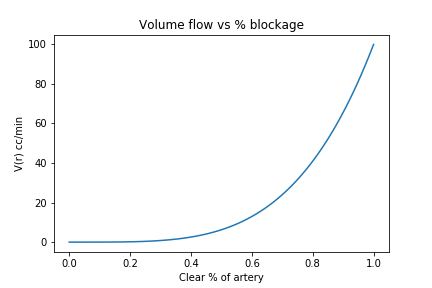
\includegraphics[scale=1]{flowvblock.png}
\end{center}
As expected, we see that the flow rate is proportional to $r^4$ as derived. As the \% of the artery that is clear increases, $r$ increases, as does the flow rate. Next, we plot the pressure needed to maintain a constant flow as a function of arterial clearness.
\begin{center}
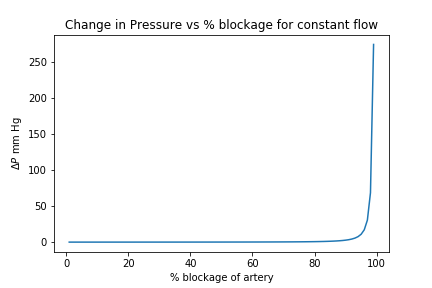
\includegraphics[scale=1]{pressureblock.png}
\end{center}
We see that this is inversely proportional to the radius. As the effective radius decreases, the overall amount of pressure grows unbounded. Eventually requiring an infinite amount of pressure on a closed vessel. Finally, we plot the peak flow rate as a function of effective radius.
\begin{center}
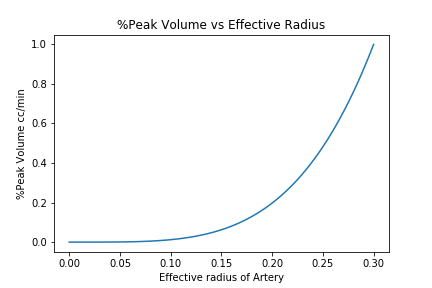
\includegraphics[scale=1]{percentpeak.png}
\end{center}
We see here that the peak flow rate is proportional to $r^4$ as expected. As the effective radius increases, the peak flow rate increases proportionally.
\end{document}
